\documentclass[12pt, titlepage]{article}

\usepackage{fullpage}
\usepackage[round]{natbib}
\usepackage{multirow}
\usepackage{booktabs}
\usepackage{tabularx}
\usepackage{graphicx}
\usepackage{float}
\usepackage{hyperref}
\usepackage{pdfpages}
\usepackage{pdflscape}

\hypersetup{
    colorlinks,
    citecolor=black,
    filecolor=black,
    linkcolor=red,
    urlcolor=blue
}
\usepackage[round]{natbib}
\usepackage{multirow}

\input{../Comments}
%% Common Parts

\newcommand{\progname}{Measuring Microstructure Changes During Thermal Treatment} % PUT YOUR PROGRAM NAME HERE
\newcommand{\authname}{Team \#30, ReSprint
\\ Edwin Do
\\ Joseph Braun
\\ Timothy Chen
\\ Abdul Nour Seddiki
\\ Tyler Magarelli
} % AUTHOR NAMES                  

\usepackage{hyperref}
    \hypersetup{colorlinks=true, linkcolor=blue, citecolor=blue, filecolor=blue,
                urlcolor=blue, unicode=false}
    \urlstyle{same}
                                


\begin{document}

\title{Verification and Validation Report: \progname} 
\author{\authname}
\date{\today}
	
\maketitle

\pagenumbering{roman}

\section{Revision History}

\begin{tabularx}{\textwidth}{p{3cm}p{3cm}X}
\toprule {\bf Date} & {\bf Developer} & {\bf Change}\\
\midrule
Date 1 & 1.0 & Notes\\
Mar. 8, 2023 & Joseph Braun & Added Sections 5, 7, 8 \\
Mar. 8, 2023 & Joseph Braun & Added Reflection \\
\bottomrule
\end{tabularx}

~\newpage

\section{Symbols, Abbreviations and Acronyms}

\renewcommand{\arraystretch}{1.2}
\begin{tabular}{l l} 
  \toprule		
  \textbf{symbol} & \textbf{description}\\
  \midrule 
  T & Test\\
  \bottomrule
\end{tabular}\\

\wss{symbols, abbreviations or acronyms -- you can reference the SRS tables if needed}

\newpage

\tableofcontents

\listoftables %if appropriate

\listoffigures %if appropriate

\newpage

\pagenumbering{arabic}

This document ...

\section{Functional Requirements Evaluation}

\section{Nonfunctional Requirements Evaluation}

\subsection{Usability}
\begin{tabular}{ |p{3cm}||p{3cm}|p{3cm}|p{3cm}|p{2cm}| }
  \hline
  \multicolumn{5}{|c|}{Usability Tests} \\
  \hline
  Requirement & Related Unit Tests & Description & Expected Result & Result\\
  \hline
  Afghanistan   & AF    &AFG&   004 & PASS\\
  Aland Islands&   AX  & ALA   &248 &\\
  Albania &AL & ALB&  008 &\\
  Algeria    &DZ & DZA&  012 &\\
  American Samoa&   AS  & ASM&016 &\\
  Andorra& AD  & AND   &020 &\\
  Angola& AO  & AGO&024 &\\
  \hline
 \end{tabular}
		
\subsection{Performance}

\subsection{etc.}
	

\section{Comparison to Existing Implementation}	

\noindent Below is an image of the exisiting implementation's GUI.

\begin{figure}[H]
\centerline{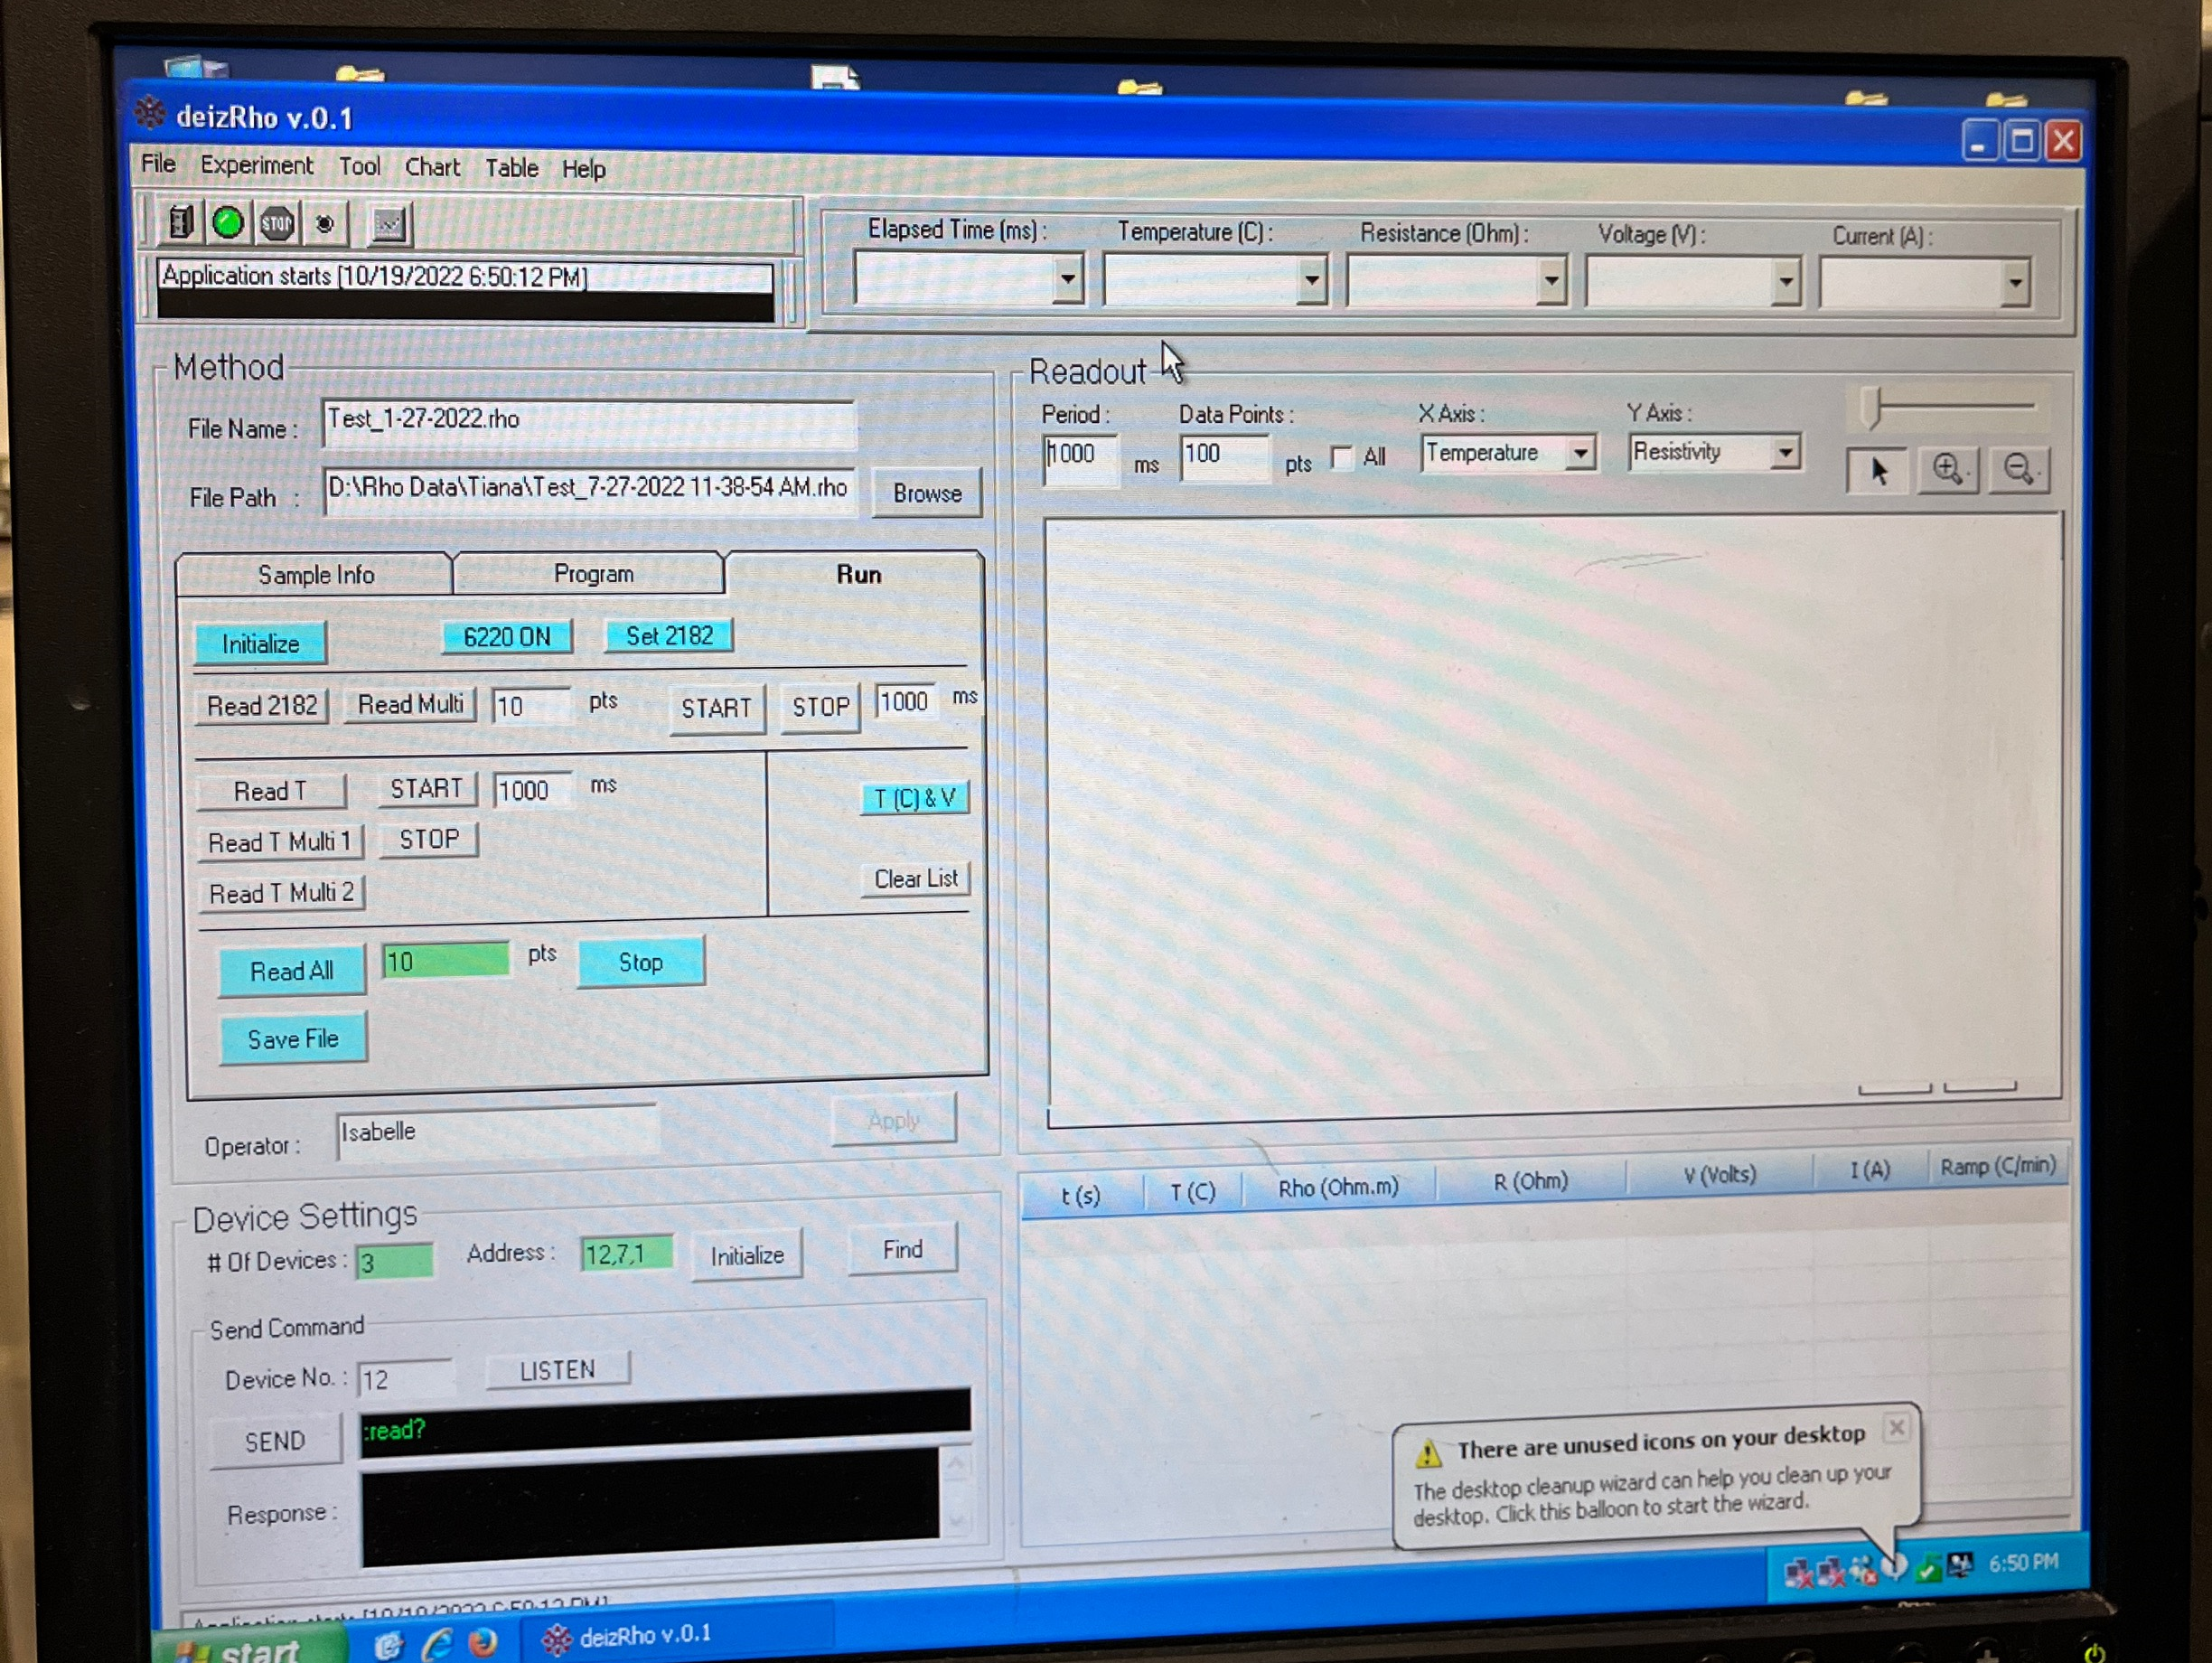
\includegraphics[scale=0.2]{app.png}}
\caption{Previous software user interface design}
\label{fig}
\end{figure}

\noindent The key elememts of the existing implementation will also be included in our implementation. This is so that the application will be familiar to the user and as intuitive as possible. These elements are listed below:
\begin{itemize}
  \item Method Panel: controls which device to read data from (temperature or voltage), and which file to save the data in
  \item Device Settings Panel: used to send SCPI commands directly to a device
  \item Readout: includes graphical output and listed output of relevant values (current, voltage, resistance, etc.)
\end{itemize}

\noindent The primary differences between the existing implementation and our implementaion are the appearance of the GUI and the option of remote access. The existing implementation was developed for Windows XP whereas our implementation is developed for Windows 10, which gives it an updated look. One of the stretch goals for this project is to enable remote access to the application to be able to monitor and stop experiments remotely. The existing implementatio  does not have this functionality.\\


\section{Unit Testing}


\section{Changes Due to Testing}

\begin{tabular}{ |p{3cm}|p{5cm}|p{5cm}| }
  \hline
  Test & Failure Observed & Change Made \\
  \hline
  Test 1 & Failed & Change made to module \\
  Test 2 & Failed & Change made to module \\
  \hline
 \end{tabular}


\section{Automated Testing}

\noindent We acheived automated unit testing through the use of the NUnit testing framework in Visual Studio. NUnit is one of the most popular test frameworks used for running tests on a .NET project.\\

\noindent NUnit tests are setup by first creating a new project file in Visual Studio and adding it to the solution file for your project (in our case, the application). In the new project file, a new class is created. Each unit test we want to carry out is written as a method of the test class. Since the project file for the test class is inlcuded in the same solution file as our application, we are able to call the test methods from our main application to run the tests.\\
		
\section{Trace to Requirements}
		
\section{Trace to Modules}		

\section{Code Coverage Metrics}

\bibliographystyle{plainnat}
\bibliography{../../refs/References}

\newpage{}
\section*{Appendix --- Reflection}

The information in this section will be used to evaluate the team members on the
graduate attribute of Lifelong Learning.  Please answer the following questions:

\begin{enumerate}
  \item In what ways was the Verification and Validation (VnV) Plan different
  from the activities that were actually conducted for VnV?  If there were
  differences, what changes required the modification in the plan?  Why did
  these changes occur?  Would you be able to anticipate these changes in future projects?  If there weren't any differences, how was your team able to clearly predict a feasible amount of effort and the right tasks needed to build the evidence that demonstrates the required quality?  (It is expected that most teams will have had to deviate from their original VnV Plan.)
\end{enumerate}

\indent There were several differences between what we had planned for VnV and what we ended up carrying out. When completing the initial revision of VnV plan, we had not yet completed the Design documents (MG, MIS, System Design) and so we did not have a plan for unit/module testing, only for system testing. Our initial VnV plan included three main sections: SRS Verification, Design Verification, and Implementation Verification.\\

\indent For SRS Verification, we planned to meet every two weeks to discuss potential updates to the SRS doc. While we continued to meet frequently (weekly or bi-weekly), our team focussed instead on the next deliverable rather than revisiting old documents during meetings. Because of this, our SRS was not continually being updated during the project. This change occurred mainly due to time constraints, as we faced some technical issues leading up to the first demo which took priority over other tasks. In hindsight, frequently revisiting and updating the SRS certainly would have created less work for us in the long run. For future projects, though we can't predict any exact technical issues that would set us back on time, we should be able to anticipate issues arising which cause delays. We should have a plan to stay on schedule despite such issues. \\

\indent  For Design Verification, we planned to use the MIS checklist to ensure that requirements in the SRS are met and hazards in the Hazard Analysis are covered. Our team followed the MIS checklist when testing. We also planned to use feedback from the course instructor, teaching assistants, classmates, and our project supervisor. There were not many changes made in this section of the plan, except that our team decided to focus primarily on feedback from Dr. Zurob, as he is the end-user of the application. \\

\indent For Implementation Verification, we planned to used GitHub issues and pull requests to maintain our code base. Any pull request made to the main branch requires at least two other team members to review and approve. We did not make any major changes to our Implementation Verification. 
\end{document}